\documentclass{VRARWorkshop}

\usepackage[utf8]{inputenc}
\usepackage[T1]{fontenc}
\usepackage[hidelinks]{hyperref}

\title{Augmented reality for supporting manual non-destructive ultrasonic testing of metal pipes and plates}

%\authors{Robert Deppe, Oliver Nemitz, Jens Herder}
\authors{~}

\affiliations{~}
% TODO: Correct affiliations

\abstract{
We describe an application of augmented reality technology for non-destructive testing of products in the metal-industry.
The prototype is created with hard- and software, that is usually employed in the gaming industry, and delivers positions for creating ultrasonic material scans (C-scans).
Using a stereo camera in combination with an {\sc hmd} enables realtime visualisation of the probes path, as well as the setting of virtual markers on the specimen.
As a part of the implementation the downhill simplex optimization algorithm is implemented to fit the specimen to a cloud of recorded surface points.
The accuracy is statistically tested and evaluated with the result, that the tracking system is accurate up to ca. 1-2 millimeters in well set-up conditions.
This paper is of interest not only for research institutes of the metal-industry, but also for any areas of work, in which the enhancement with augmented reality is possible and a price tracking is necessary.
}

% Give some keywords
\keywords{
Nondestructive Testing,
Ultrasonic,
Augmented Reality,
Tracking,
Stereo camera,
head mounted display,
NDT,
AR
}

\begin{document}

\section{Introduction}

In the field of nondestructive testing of steel products, the ultrasonic (US) inspection is a frequently used method to assure given safety requirements \cite{deutsch_zfp_2010} \cite{moles_introduction_2004}
\cite{olympus_Grundlagen}.
For heavy plates and large diameter pipes the manual US testing is often applied as a follow-up inspection. Here, a US probe is moved by hand on the surface of the specimen (Figure \ref{fig:manual_UT}). While moving and possibly rotating the probe the operator monitors the US signal on a screen. Usually, in case of an imperfection in the material, the US signal exhibits a higher amplitude and the position of the imperfection can be marked on the specimen.
However, the exact position and orientation of the probe are not captured during the manual inspection. Hence, generating an objective report with for example a map of color coded US amplitudes onto probe positions (a so-called C-scan, cf. Figure \ref{fig:cScan}) is not directly possible.
Furthermore, those parts of the specimen surface that have already been inspected are usually not tracked and visualized.
There is especially no control if there is a gap in the inspection path. \\
The aim of our system is therefore to track the position and orientation of the US probe during the inspection and assign them to the corresponding US signals. This tracking is done with standard AR/VR components of an HTC VIVE system. The probe is attached to a VIVE tracker and the global coordinates of the probe are converted to coordinates in a local coordinate system on the specimen. These local coordinates are sent to a UT inspection software which generates a C-scan of the specimen.
By a ZEDmini stereo camera it is possible to view the inspection in AR and to visualize certain virtual elements as for example the pathes of the already inspected areas. \\
In this work only plate products have been considered, i.e. specimen with planar surfaces. In a subsequent step it is planned to extend this work to pipes, i.e. cylinder shaped specimen.

\begin{figure}[h!]
    \begin{center}
        \includegraphics[width=0.8\textwidth]{images/US-workspace}
        \caption{\label{fig:manual_UT} Manual ultrasonic testing of steel large diameter pipes.}
    \end{center}
\end{figure}
\begin{figure}[h!]
    \begin{center}
        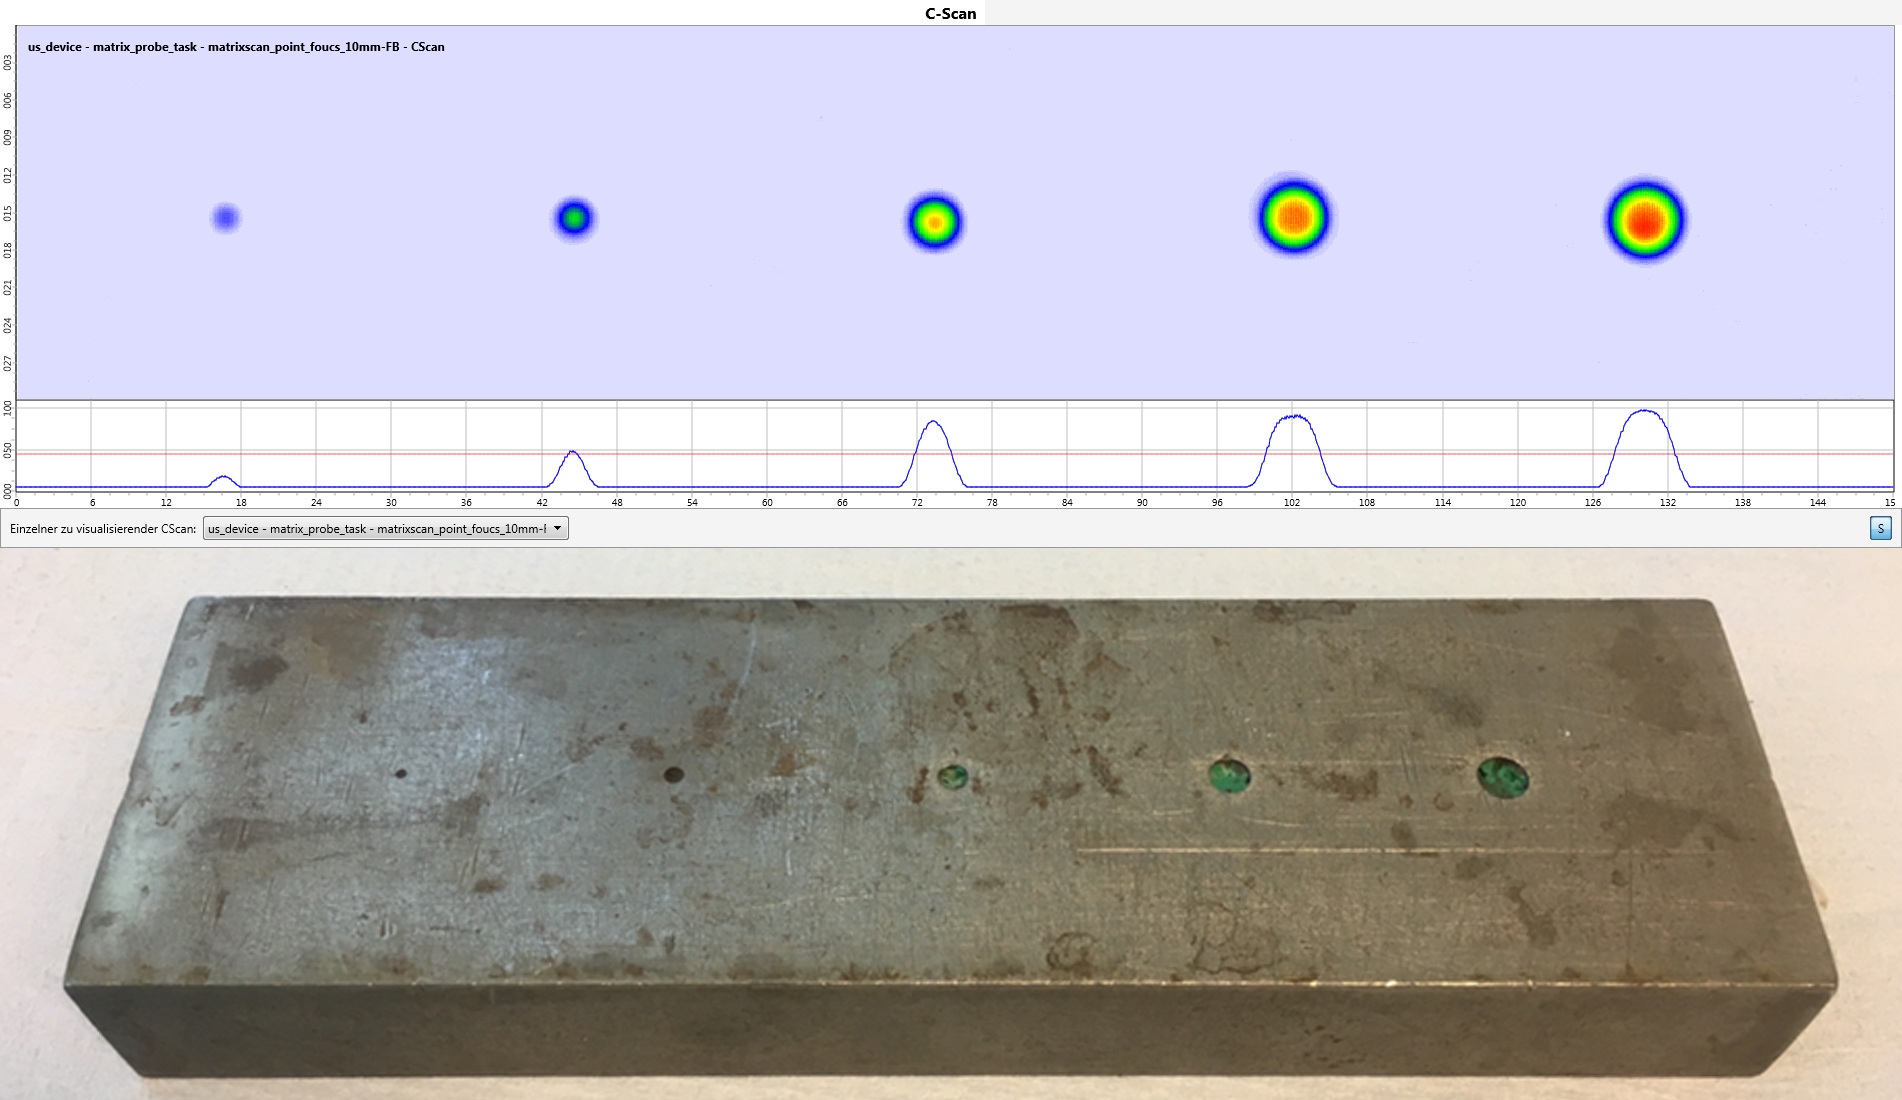
\includegraphics[width=0.8\textwidth]{images/CScan}
        \caption{\label{fig:cScan} Example of a C--Scan: A plate specimen (top) with multiple flat bottom holes of different diameters has been inspected with a 5 MHz probe which has been moved along a rectangular grid across the back side. At each grid position an amplitude value is extracted from the US signal and converted to a color. The resulting image on the grid is the so-called C-scan which can be seen at the bottom.
				Here, a rectangular grid with a fine resolution of 0,1\,mm has been used.}
    \end{center}
\end{figure}

\section{Related Research}
In the 2015 released patent \textit{A system and method of non-destructive inspection with a visual scanning guide} \textit{Olympus} patented the procedure of enhancing the manual inspection with AR-Glasses which help to trace a predefined inspection-plan path.
The patent describes details like tolerated deviation from the inspection path.
However there is no mentioning of the possibility to log specific points or the traced path on the probe \cite{ARPat15}.\\

The article \textit{Non-contact tracking of phased-array probe and real-time generation of C-scans for the inspection of composite aerospace structures} describes a system, which uses a stereo camera and active markers to determine the probes position and orientation on a possibly curved surface of plane components \cite{walter_non-contact_2007}.\\

A similar system, supporting the cleaning of surfaces is presented in the article \textit{Cleaning Up With Augmented Reality} by Alice Bonasio.
It describes the advantages of using AR-technology, like a DRAW or HYBRID system (section~\ref{sec:DrawVsErase}), can have on quality assurance in the commercial cleaning industry \cite{ARClean}.\\

The article \textit{Design, simulation, and kinematic analysis of a manipulator-based 3D position tracking system} describes a manipulator based system to track the position and orientation of B-scans in a medical application of ultrasonic inspection to create three dimensional voxels of the measurement values.
\cite{fadzil_design_2015}\\


\section{Description of the AR--application}
The AR--application supports manual US testing in two ways. First,
the operator is able to see the already inspected path and identify gaps through a AR-{\sc HMD}.
Futhermore, it is possible to visualize the axes of the local coordinate system on the specimen as well.
For these AR visualizations, a \textit{ZEDmini}, a stereo camera that can be used to display a camera image in the {\sc HMD} and to create a depth mask, has been attached to the {\sc HMD} \cite{dorner_virtual_2013}. \\
Second, the position and rotation of the probe are sent to the ultrasonic scanning computer.
There, the data is combined with the measurements received by the probe and a C--Scan can be
generated.

\section{Implementation}
The AR-application was implemented in the game engine Unity. The application cares about defining a local coordinate
system on the specimen and about receiving
global coordinates from the VIVE basestations
and converting them into local coordinates.
These local coordinates are transferred by TCP/IP to a US inspection software written by SZMF.
The US inspection software combines them with the US signals that have been received
at the same time. The US signals can be further processed into a C-scan or other result types.
The whole setup is illustrated in Figure \ref{fig:Setup}. \\

\begin{figure}[h!]
    \begin{center}
        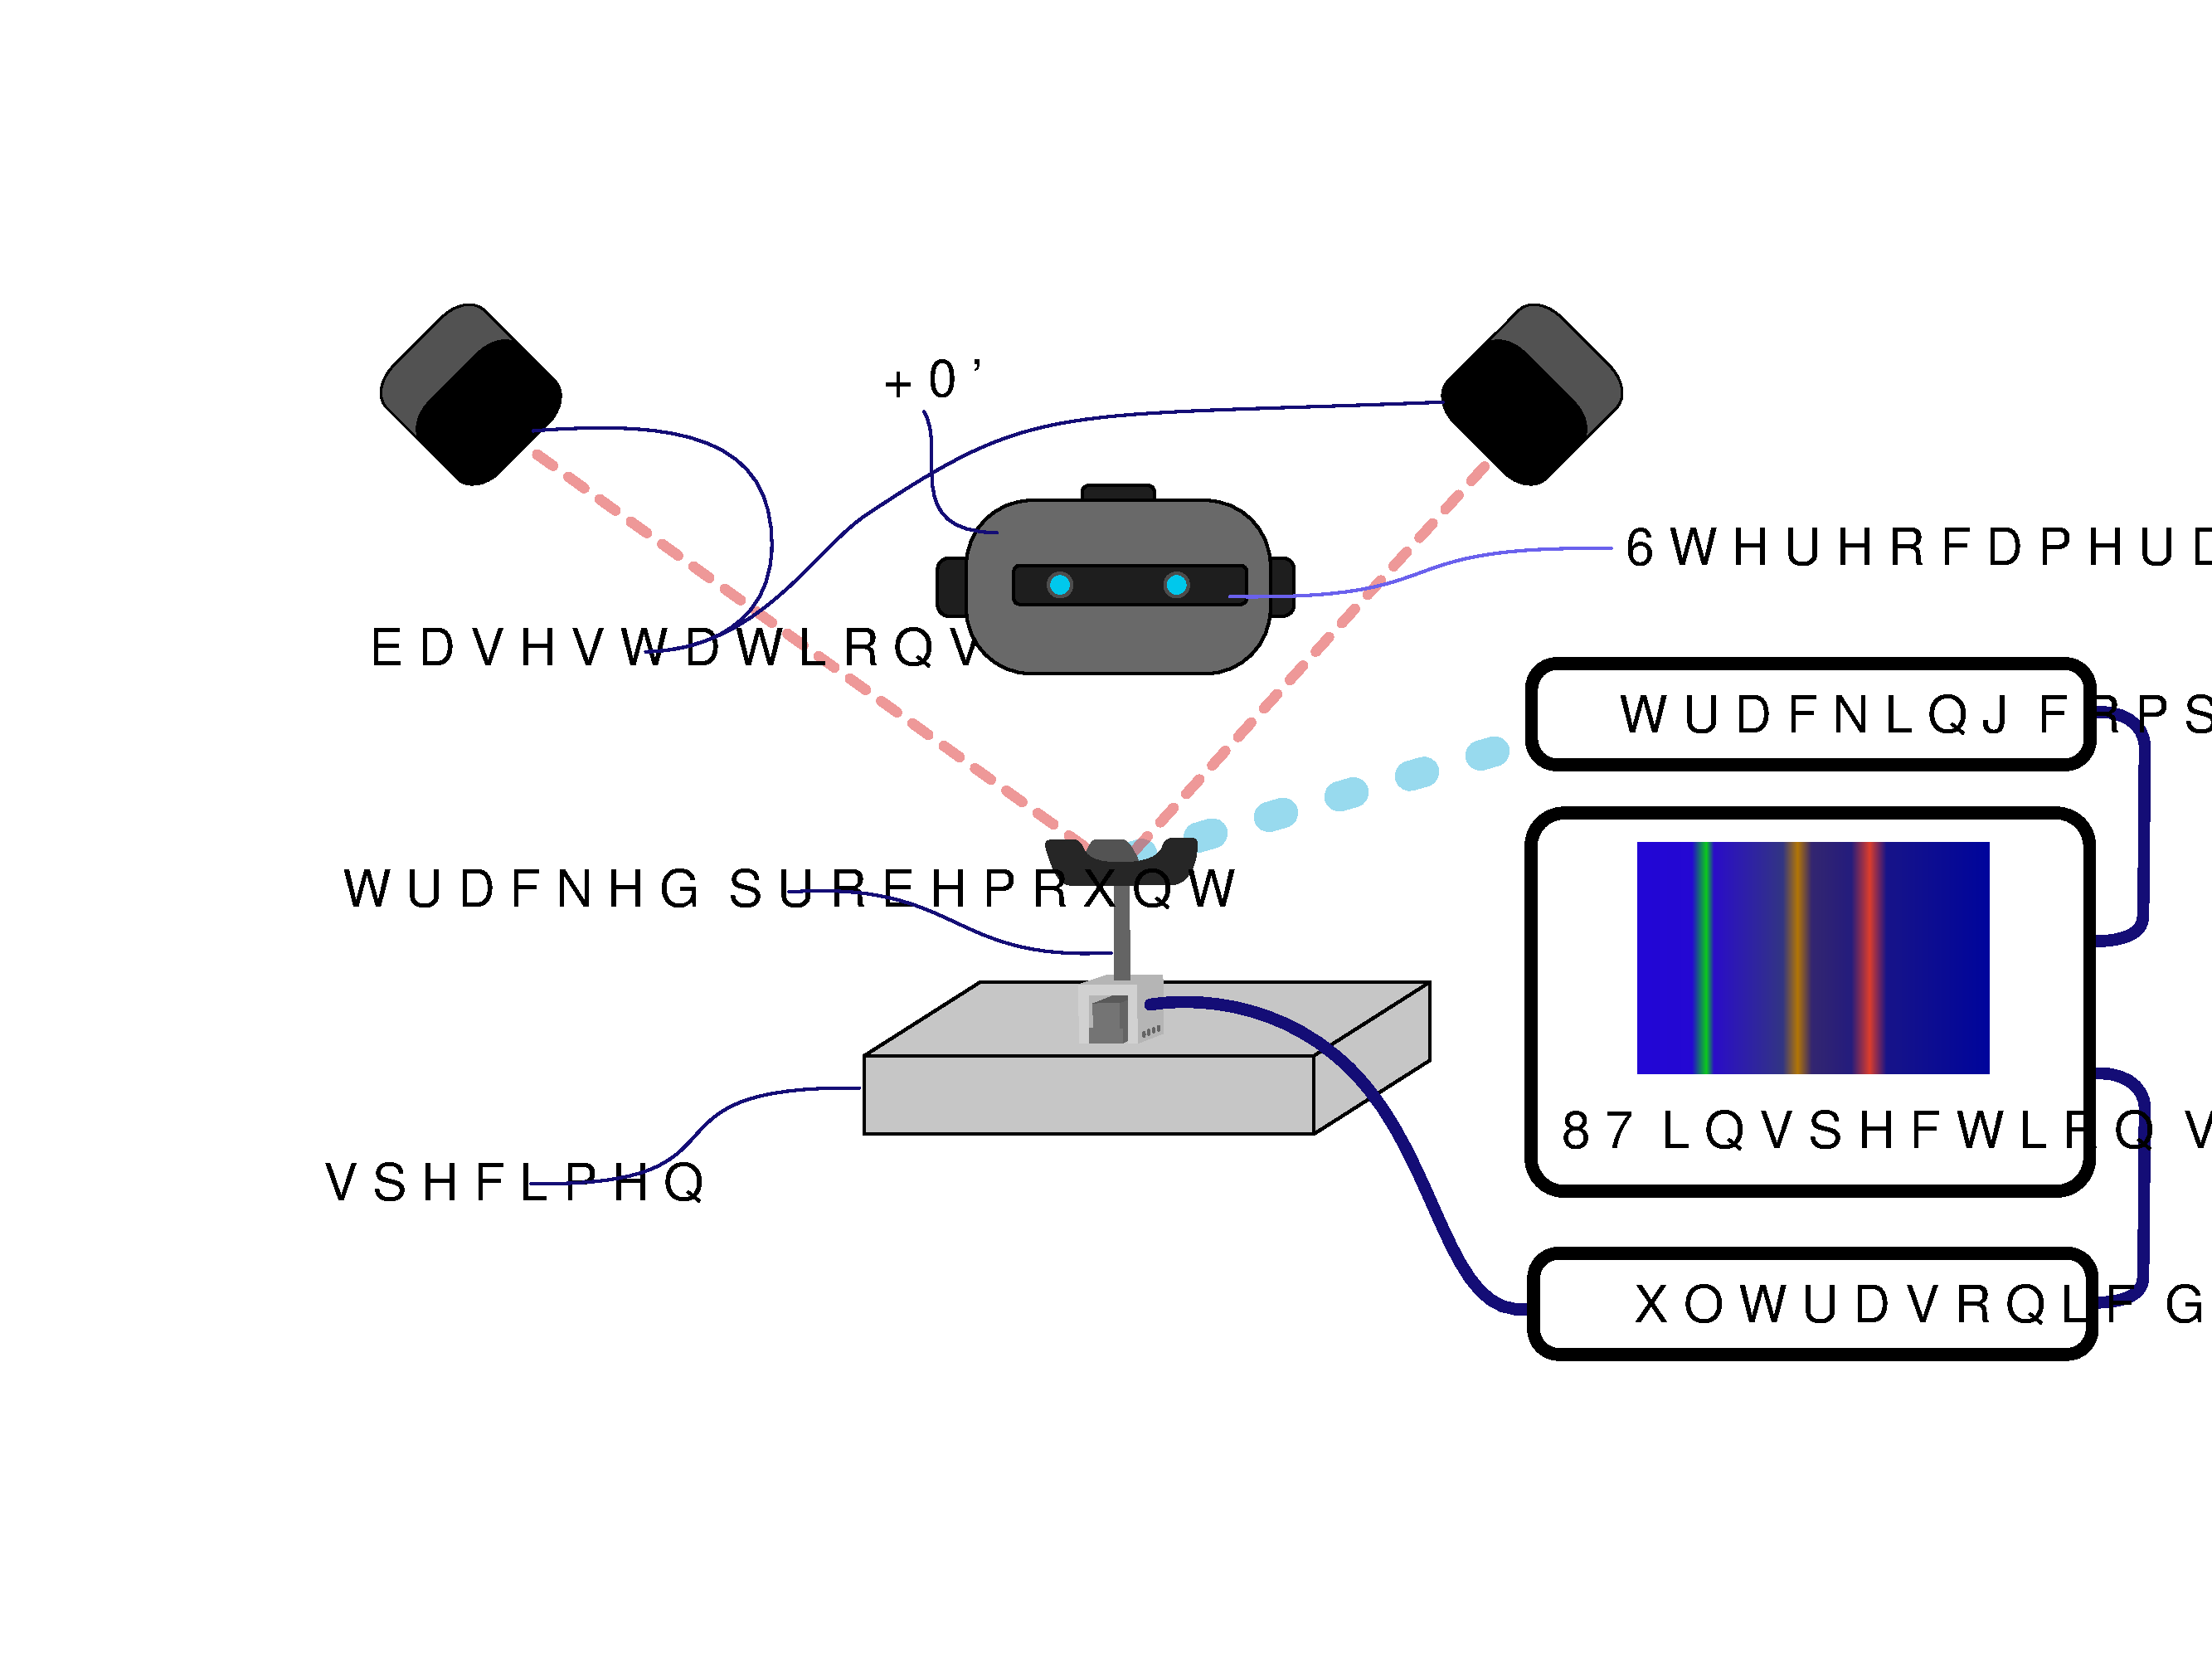
\includegraphics[width=158mm]{images/Setup-ARUS}
        \caption{\label{fig:Setup} Setup of the described AR-application.}
    \end{center}
\end{figure}

\subsection{Tracking of the ultrasonic probe}
The ultrasonic probe is tracked with the help of an attachable tracked \textit{VIVE} tracker.
This tracker is attached to a mount, in which the ultrasonic probe is fixed (Figure~\ref{fig:AR-table}).

The offset and orientation between the tracker and probe is applied in software by setting the virtual probe as a child transform of the tracker.

\subsection{Detection of the coordinate system in worldspace}
The local coordinate system of the surface to be measured is defined in two steps:
first a point--cloud of the surface is created by moving the tracked probe across it.
In the next step a plane is fitted into this point--cloud using the Downhill--Simplex optimization by Nelder and Mead. For the planar specimen considered in this work a simple plane computation based on three measured points
would be possible, too. But for later applications on pipes and other geometries, such a fitting algorithm usually works more stable. \\
In a second step the local coordinate system is determined by defining its origin and the direction of the X-Axis.
The Y-Axis in the fitted plane is then automatically chosen orthogonally to the X-Axis and the Z-Axis is the vector product of the X- and Y-Axis.
In the application, the origin and the direction of the X-Axis are chosen by pressing the setup button.


\subsection{Visualization of the tracking-data}
\label{sec:DrawVsErase}
To visualize the already traced path, a visual feedback is given to the operator.
The feedback can be implemented in multiple ways, depending on the application.
The path can either be drawn on the surface ({\sc Draw}), erased from a pre-colored area ({\sc Erase}), or be drawn onto a pre-colored area ({\sc Hybrid}) (Figure~\ref{fig:DrawVsErase}).

\begin{figure}[h!]
    \begin{center}
        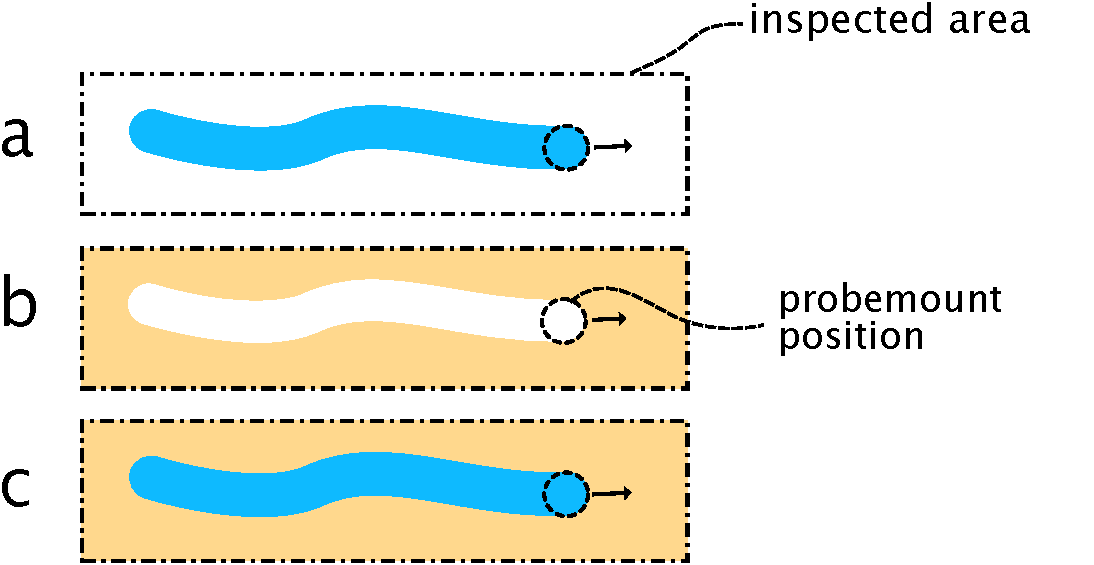
\includegraphics[width=79mm]{images/DrawVsErase}
        \caption{\label{fig:DrawVsErase} Different methods to mark covered area. (a) {\sc Draw} (b) {\sc Erase} (c) {\sc Hybrid}}
    \end{center}
\end{figure}

The main purpose of this visualization is to show possible gaps in the inspection, or to follow a predefined inspection-path.
In the case of SZMF, there is usually no specific inspection-plan that can give a pattern to erase, therefore {\sc DRAW} was implemented.
The AR-view of the application can be seen in Figure~\ref{fig:ARView}.

\begin{figure}[h!]
    \begin{center}
        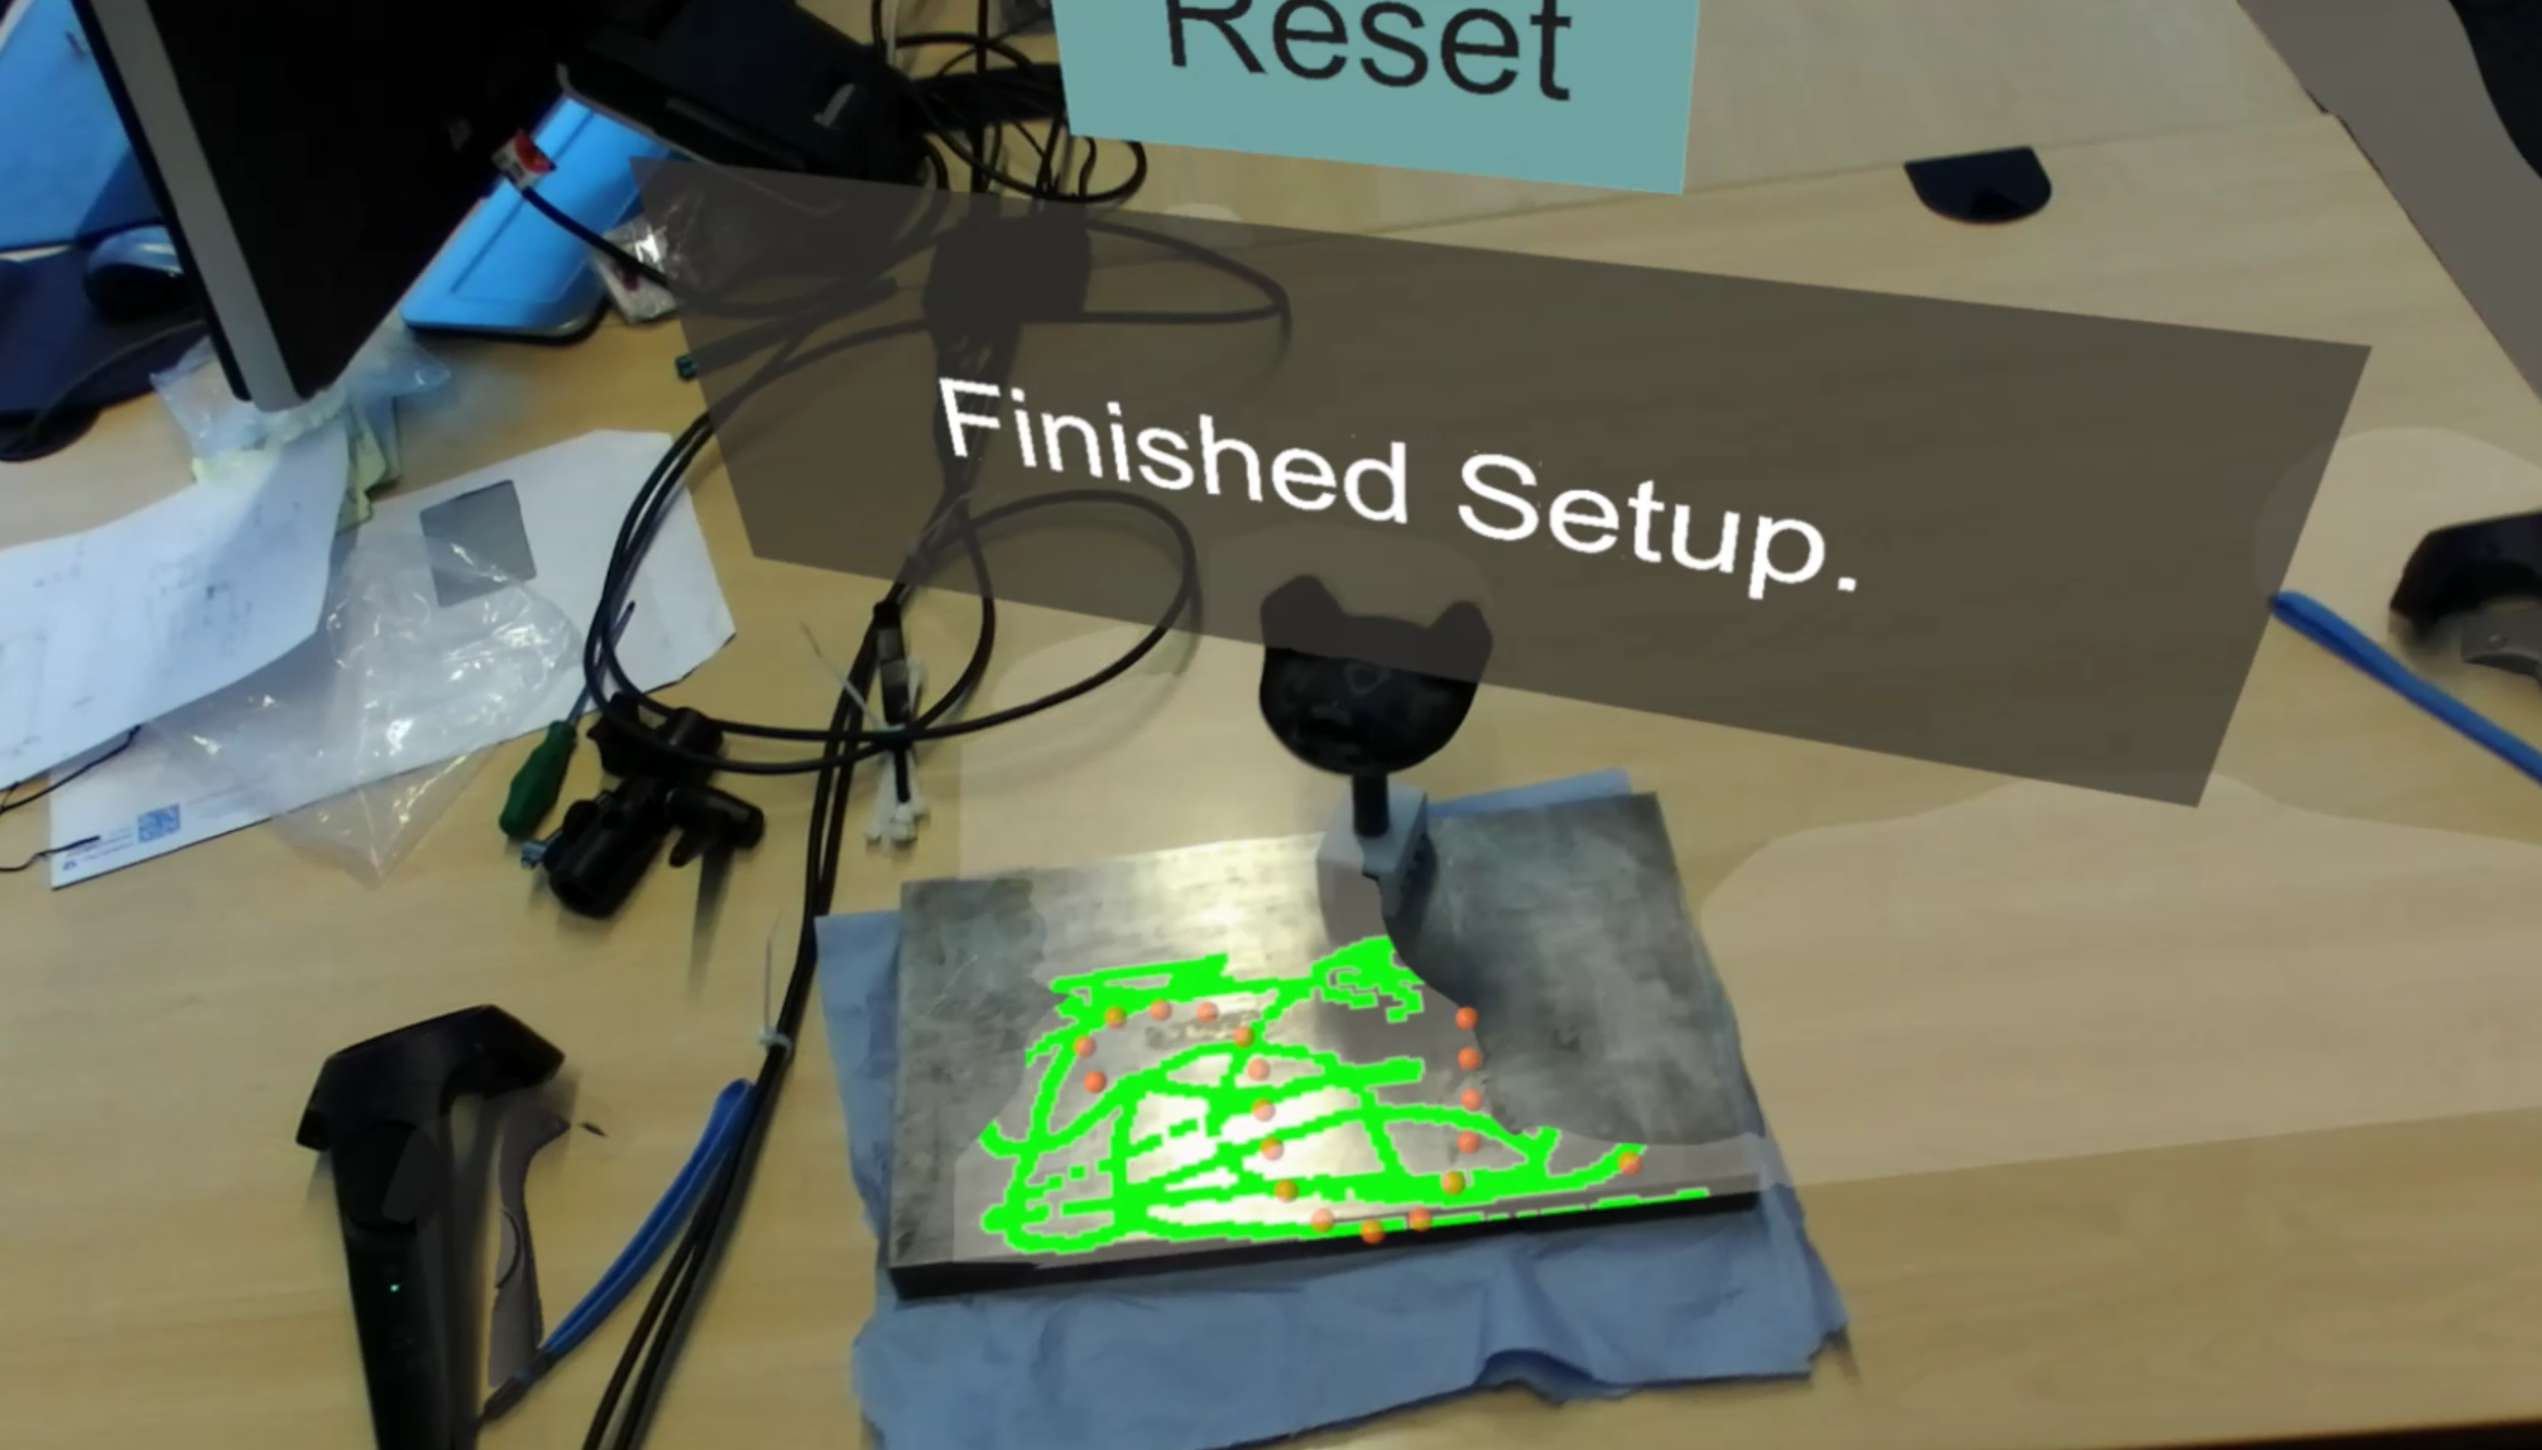
\includegraphics[width=90mm]{images/AR-Screenshot}
        \caption{\label{fig:ARView} AR-view of the application with green drawn path, the probe has covered.}
    \end{center}
\end{figure}

The patches in the surface, where no color can be seen, can be explained by a lack in accuracy of the depth image, generated by the used stereocamera.

\subsection{Results}

(figure~\ref{fig:AR-table})

\begin{figure}[h!]
    \begin{center}
        \includegraphics[height=60mm]{images/ARUS-table-croped}
        \caption{\label{fig:AR-table} Left: Setup of the system with live generated C-scan visible on the monitor. Right: Probemount used in the }
    \end{center}
\end{figure}

\subsection{Continuous and singular logging of position}
The application allows the continuous logging of the probes position.
This protocol can be useful for documenting exactly which path was taken, and where exactly the imperfections were detected.
In addition to that, it is possible to log singular spots and store them for later use.

\section{Evaluation of the \textit{VIVE}-tracker accuracy}
The accuracy of the \textit{VIVE}-Tracker was determined in a experiment using an automated X-Y-scanner.
Both \textit{VIVE}-Basestations were positioned on opposite corners of the scanner, though one at a greater distance (figure~\ref{fig:precisionMeasurementSetup}).

\begin{figure}[h!]
    \begin{center}
        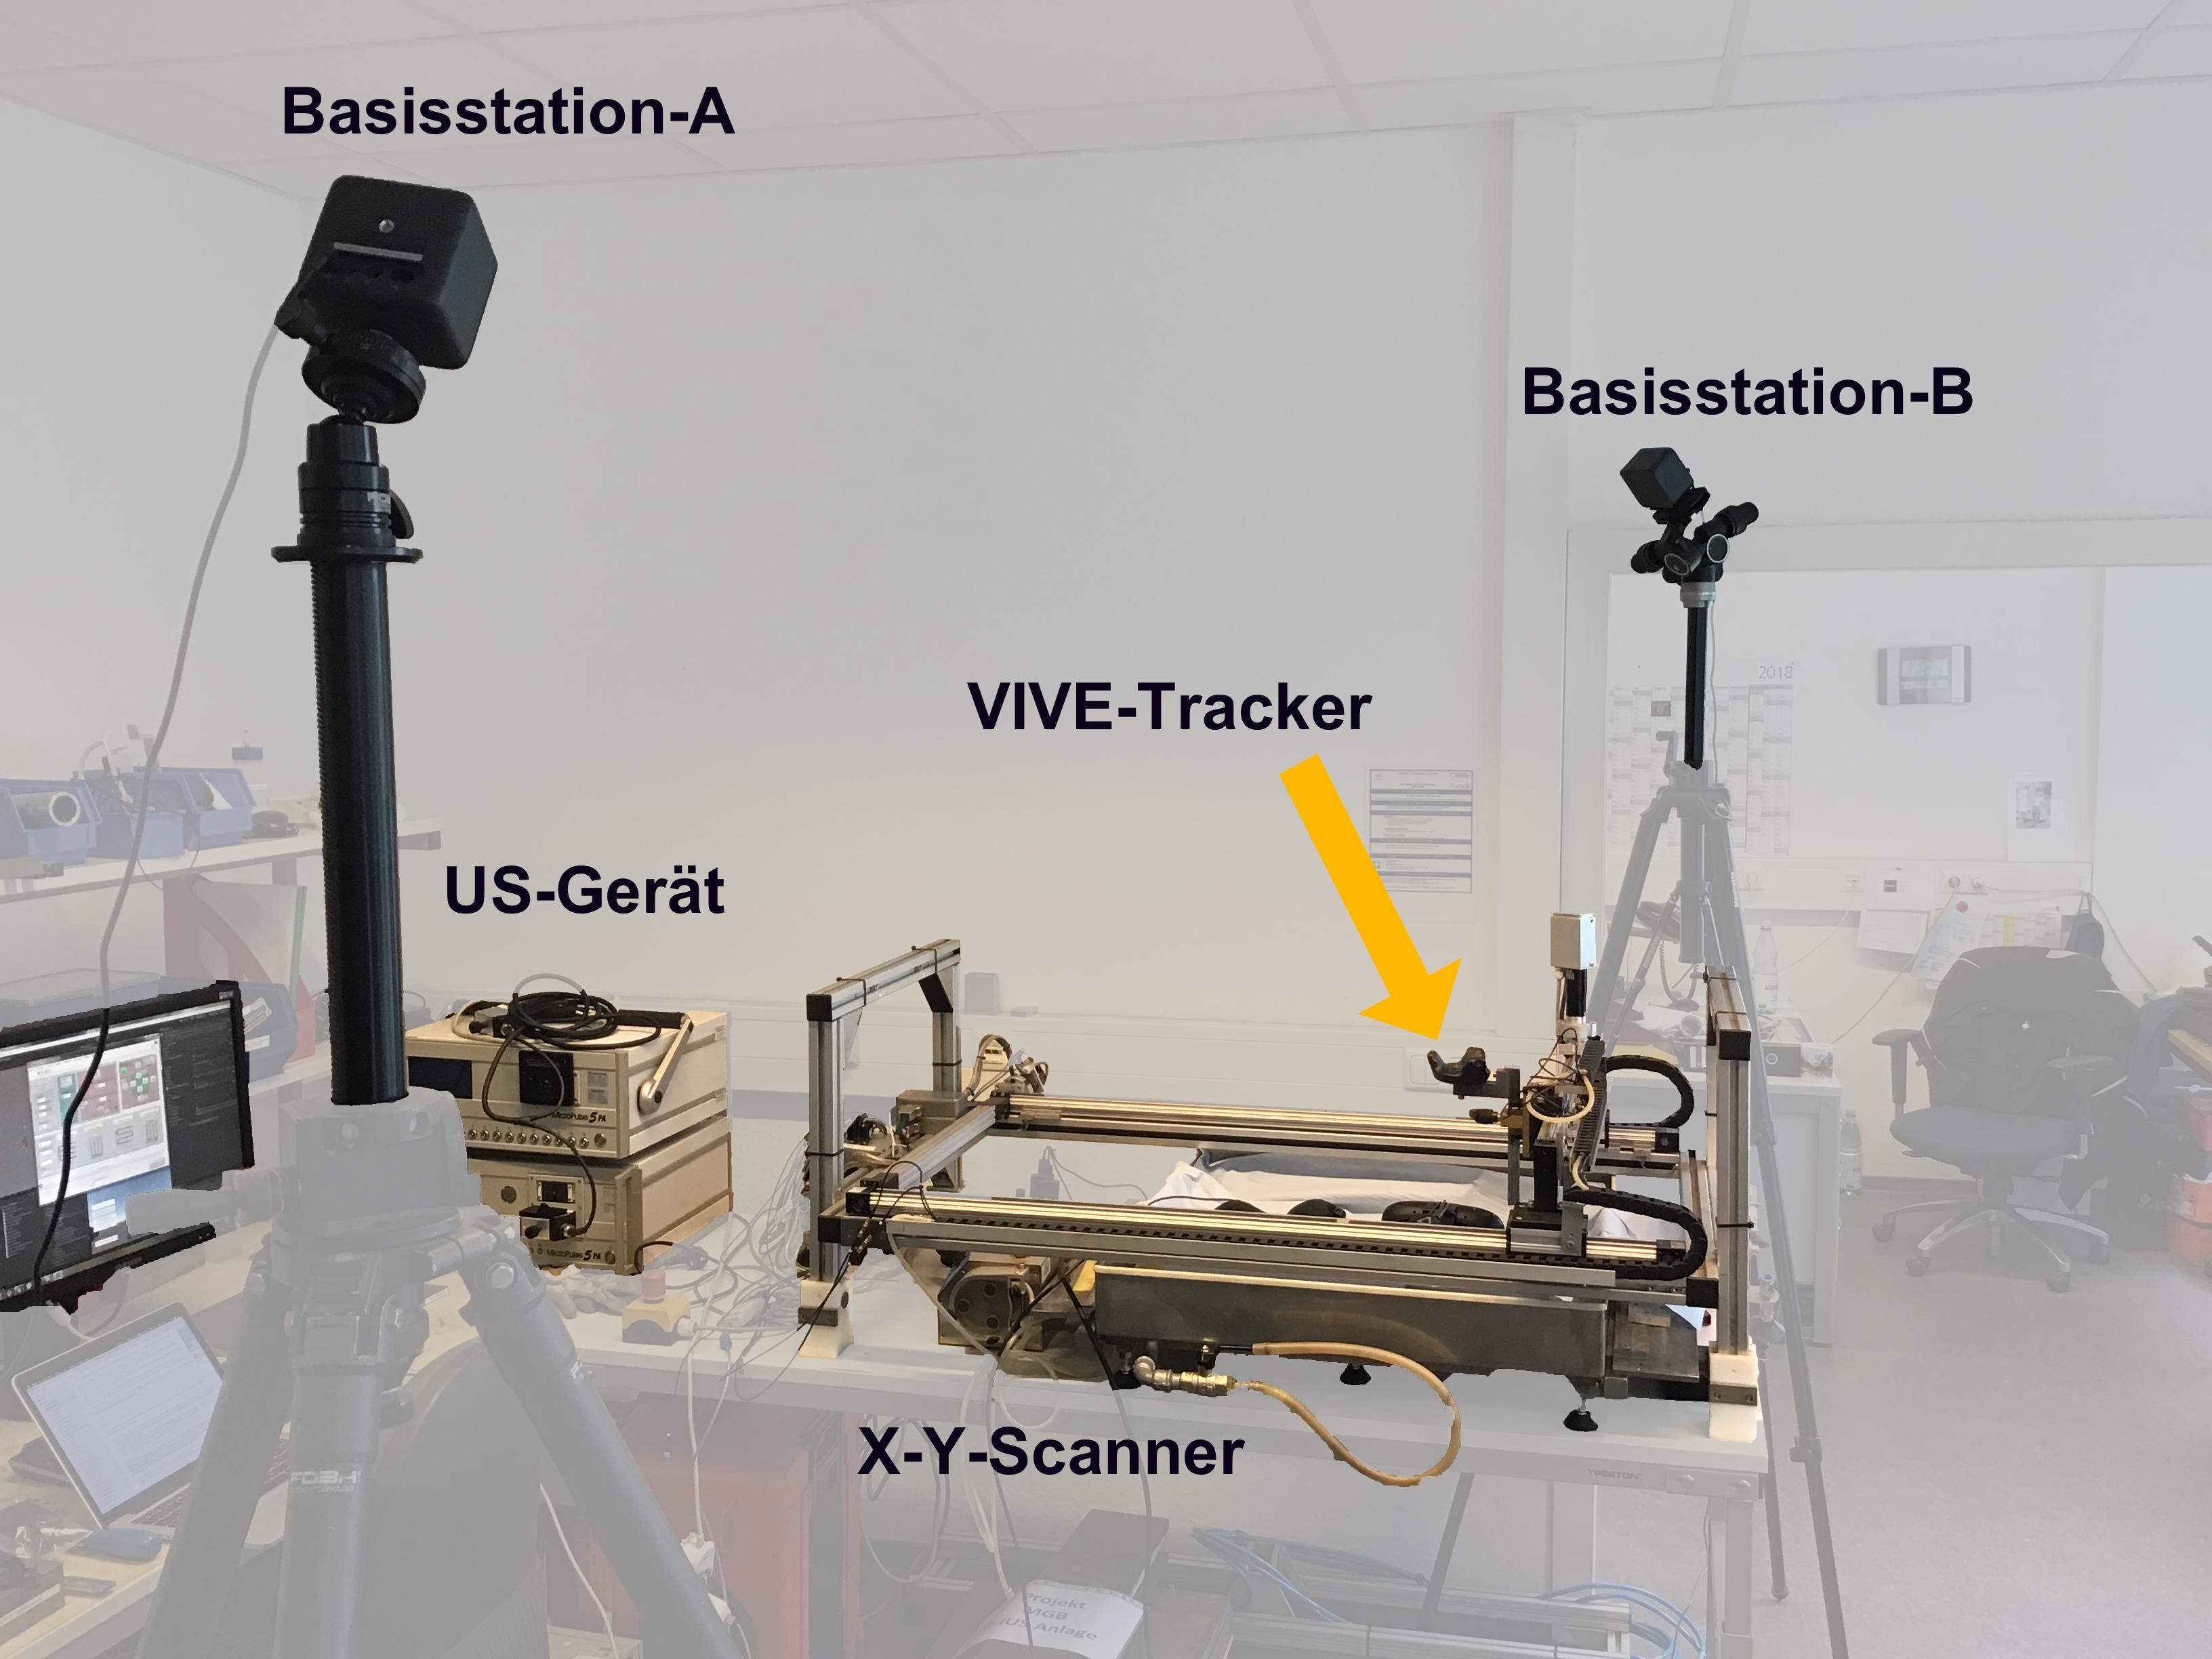
\includegraphics[width=120mm]{images/PrecisionMeasurement}
        \caption{\label{fig:precisionMeasurementSetup} Setup for the evaluation of the \textit{VIVE}-Precision.}
    \end{center}
\end{figure}

The results show a decline in quality as the surveypoints get closer to the closer basestation (basestation-B in figure~\ref{fig:precisionMeasurementSetup}) with an error up to 18\,mm.
In the opposite corner the values had a quality of about 1-2\,mm.
This can be explained by the rapidly declining quality as the proximity to the basestation is too small.

\section{Conclusion}

\begin{figure}[h!]
    \begin{center}
        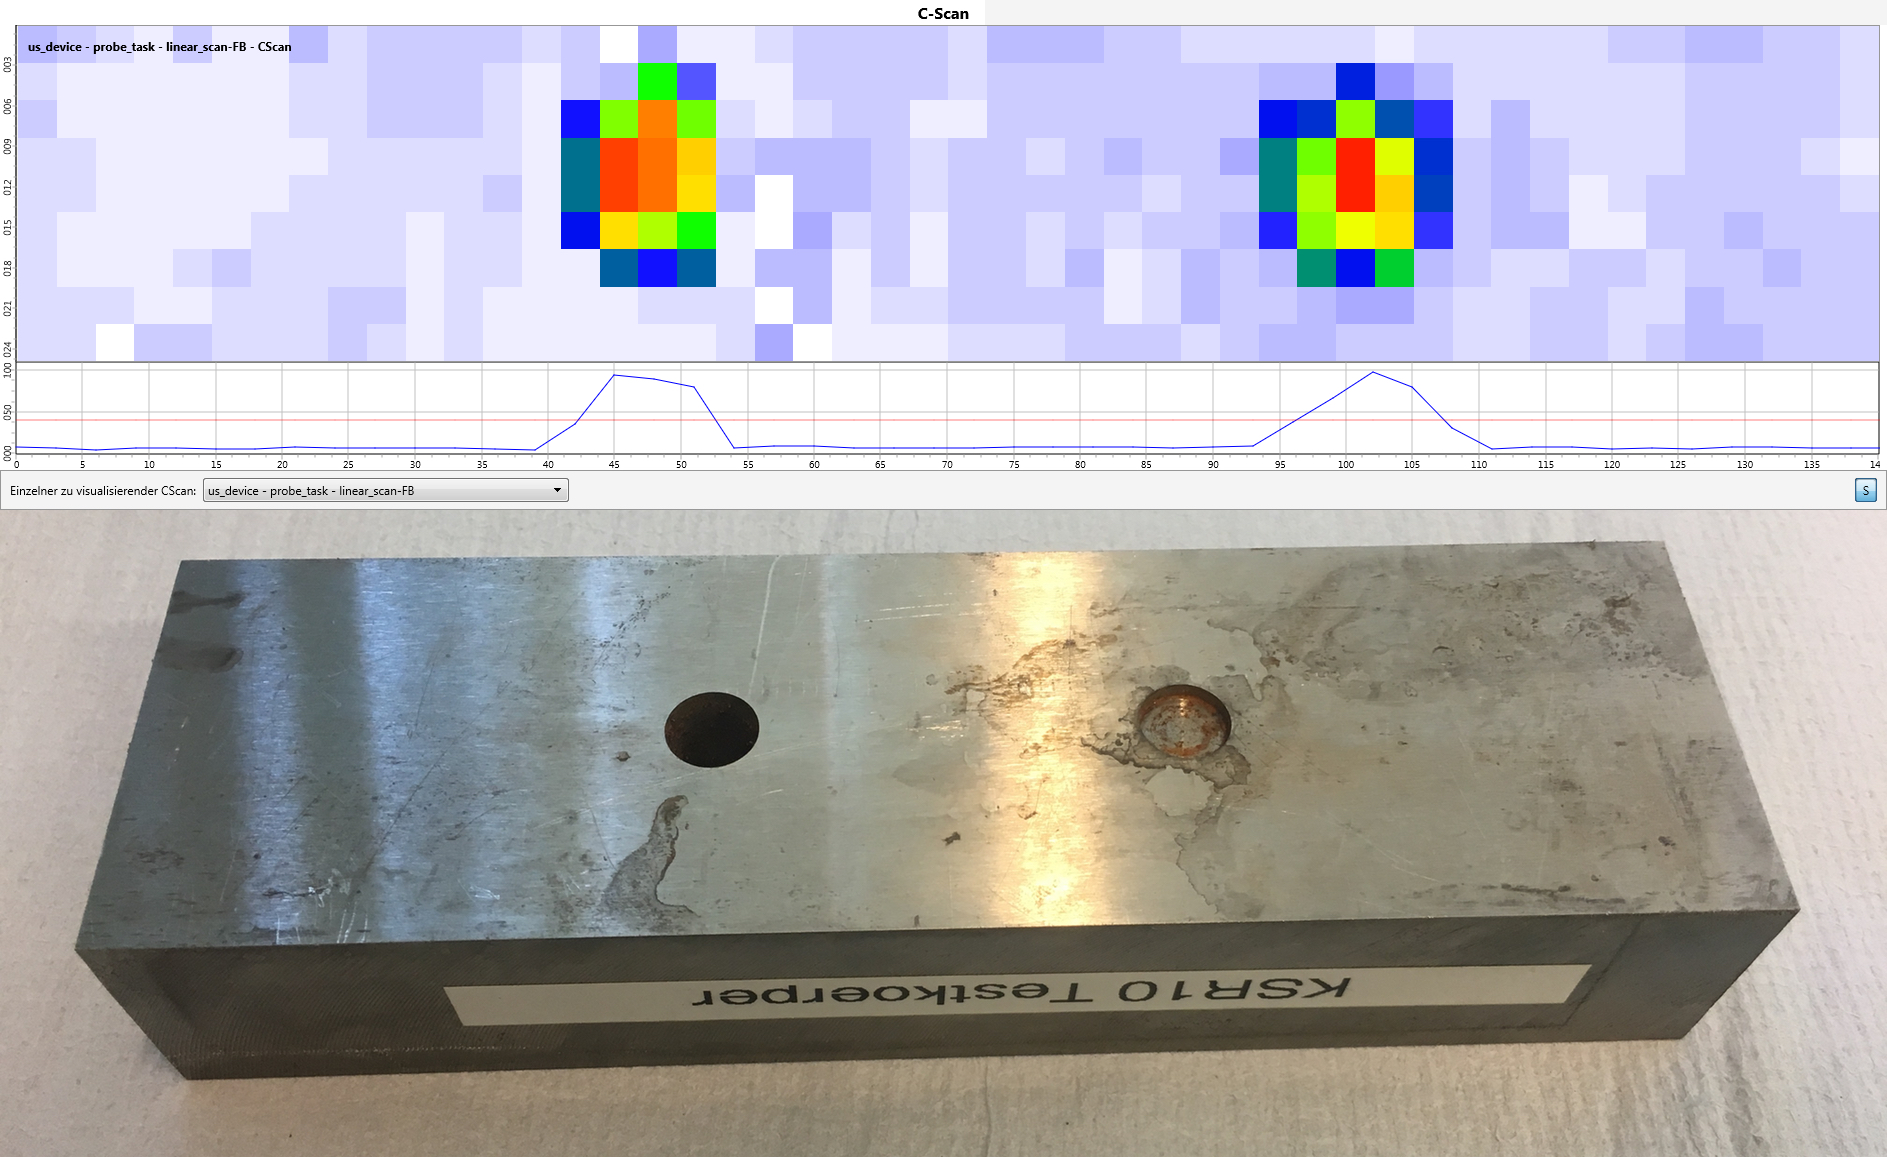
\includegraphics[width=100mm]{images/CScanARUS}
        \caption{\label{fig:resultCScan} C-scan generated with the \textit{VIVE}--tracking system}
    \end{center}
\end{figure}

We have used a VR-Tracking system, which is ordinary used for {\sc hmd} applications, for tracking an ultrasonic sensor.
We showed that the accuracy for generating ultrasonic volume images is good enough (Figure~\ref{fig:resultCScan}), enabling cost effective systems.
The {\sc hmd} system was modified with a stereo camera for building an AR video-see-through system.
AR was used to show an operator the manual scanned surface.
The developed registration procedure for the test object allows multiple measurement on different occasion.
In the application field an object will be tested, modified and repaired, and finally tested again.
The final test will be done for the same measurement area, which can be found through the registration method.
The developed prototype is not mobile and robust enough to be used in the field, but with the advances in AR displays and mobile tracking, improved nondestructive testing procedures for advanced product quality can be developed.

\VRARsetbibstyle
\bibliography{bibliography}

\end{document}
